\newcommand{\TeamNo}{31}

\newcommand{\HWno}{03}

\newcommand{\AuthorOneName}{Merve Nur Öztürk}
\newcommand{\AuthorOneID}{2311322}

\newcommand{\AuthorTwoName}{Atakan Süslü}
\newcommand{\AuthorTwoID}{2311371}

\newcommand{\AuthorThreeName}{Betül Rana Kuran}
\newcommand{\AuthorThreeID}{2311173}


\documentclass[letterpaper,12pt]{article}
\usepackage{tabularx} % extra features for tabular environment
\usepackage{amsmath}  % improve math presentation
\usepackage{amssymb}
\usepackage{xcolor}
\usepackage{float}
\usepackage[export]{adjustbox}
\usepackage{graphicx} % takes care of graphic including machinery
\usepackage[margin=1in,letterpaper]{geometry} % decreases margins
\usepackage{cite} % takes care of citations

\begin{document}
\begin{center}
AE 305, 2020-21 Fall \hfill \textbf{HW \HWno} \hfill \textbf{Team \TeamNo} \\
\noindent\rule{\textwidth}{0.4pt}
\begin{tabular}{p{0.33\textwidth} | p{0.33\textwidth} | p{0.33\textwidth} }
	\AuthorOneName&\AuthorTwoName&\AuthorThreeName\\
	\textit{\AuthorOneID}&\textit{\AuthorTwoID}&\textit{\AuthorThreeID}
\end{tabular}
\noindent\rule{\textwidth}{0.4pt}
\end{center}

%Report start

\section{Introduction}
\label{section:intro}

Finite Volume Method is a numerical method used in order to solve partial differential
equations representing the conservation of a quantity. In this homework, potential flow
field over a circular cylinder at various values of angle of attack and a symmetric NACA
airfoil at zero angle of attack is requested to be calculated. For a potential flow,
velocity field is obtained by the Laplace's equation:

\begin{equation}
	\vec{\nabla} \cdot \vec{\nabla}\phi = \frac{\partial^2 \phi}{\partial x^2} + \frac{\partial^2 \phi}{\partial y^2} = 0.
\end{equation}

\begin{equation}
\vec{V} = \vec{\nabla}\phi
\end{equation}

A pseudo time derivative is introduced in order to solve this equation without a system
of linear algebraic equations.

\begin{equation}
	\frac{\partial \phi}{\partial t} = \nu \left(\frac{\partial^2 \phi}{\partial x^2} + \frac{\partial^2 \phi}{\partial y^2}\right)
\end{equation}

where $\nu$ is an artificial diffusion coefficient. Steady state boundary conditions are
set to calculate the steady state solution as the time derivative goes to zero during the
integration. The integral form of the above equation is:

\begin{equation}
	\frac{\partial}{\partial t} \int_{\Omega}\phi  d\Omega + \oint_{S} \vec{F} \cdot d\vec{S} = 0
\end{equation}

\begin{equation}
	\vec{F} = -\nu\frac{\partial \phi}{\partial x}\vec{i} - \nu\frac{\partial \phi}{\partial y}\vec{j}
\end{equation}

Two boundary conditions are set such that the velocity is equal to the free stream velocity
far away from the body (Farfield BC) and there is no flow normal to the body, which is no
penetration boundary condition (Wall BC):

\begin{eqnarray}
	\vec{\nabla}\phi|_{far BC} &=& \vec{V}_{\infty} = \vec{u}_{\infty}\vec{i} + \vec{v}_{\infty}\vec{j} = V_{\infty}(cos\alpha\vec{i}+sin\alpha\vec{j})\\
	&=& V_{\infty}cos\alpha\vec{i} + V_{\infty}sin\alpha\vec{j}
\end{eqnarray}

\begin{equation}
	(\vec{n}\cdot\vec{V}_{\infty})_{wall} = 0 or (\vec{F}\cdot\vec{S})_{wall} = 0.
\end{equation}

The conserved quantity for this problem is the potential $\phi$, and the FV method is applied
for the calculation of this quantity as explained above.



\section{Method}
\subsection{Finite Volume Method} 
In this homework, Finite Volume Method is used. In this method, an integral conservation law
\begin{equation}
        \frac{\partial}{\partial t}\int_{\Omega_e} q\,d\Omega + \oint_{S_e} \vec{F} \cdot \vec{dS} =0     
        \label{eqn:fvm}
\end{equation}
is applied to each control volume $\Omega_e$, and its boundries $S_e$ in a discrete form. First, solution domain is divided into small triangular cells and a computational mesh is created. 
Then, all cells are labeled and neighbour cells to their surfaces are identified. Then, conservation law is applied to all cells.\\
A pseudo time derivative is substituted into Laplace equation which is multiplied by artificial 
diffusion coefficient,$\nu$. The equation becomes
\begin{equation}
        \frac{\partial \Phi}{\partial t} - \nu \vec{\nabla}\cdot\vec{\nabla}\Phi = 0
        \label{eqn:pseudodiff}
\end{equation}
where $\vec{F}=-\nu\vec{\nabla}\Phi$\\
Since a steady state solution is obtained as the derivative goes to zero and steady boundry conditions 
are specified,Laplace’s equation is satisfied. 
The integral form of Equation \ref{eqn:pseudodiff} becomes
\begin{eqnarray}
        \frac{\partial}{\partial t}\int_{\Omega} \Phi\,d\Omega + \oint_S \vec{F} \cdot \vec{dS} =0\ \\
        \mbox{where}\: \vec{F}=f\vec{i}+g\vec{j}=-(\nu\frac{\partial \Phi}{x}\vec{i}+\nu\frac{\partial \Phi}{y}\vec{j})\nonumber
        \label{eqn:genel}
\end{eqnarray}
Equation \ref{eqn:fvm} and Equation \ref{eqn:genel} have the same form. Therefore, finite volume method can be applied.\\
A simple discete form of the Equation \ref{eqn:genel} applied to a two dimensional triangular cell $e$ is then given by
\begin{equation}
        \frac{d(\Phi_e\Omega_e)}{t}+\sum_{s=1}^{3} (\vec{F} \cdot \vec{dS})\ =0
        \label{eqn:diff}
\end{equation}
where $\Phi_e$ is the average $\Phi$ over element e, $\Omega_e$ is the area of triangle $e$ ,and
$\vec{S} = \Delta y_{e,s}\vec{i}-\Delta x_{e,s}\vec{j}$\\
In this homework, averaging of cell-based quantities approach is used to calculate flux values. According to this approach,
it should be taken that averages of the cell-based flux values of the cells sharing the same surface to compute the flux 
through this surface.Therefore, the second term of \ref{eqn:diff} becomes
\begin{eqnarray}
	\sum_{s=1}^{3} (\vec{F} \cdot \vec{dS})&=&\sum_{s=1}^{3} (\vec{F_{e,s}} \cdot \vec{dS_{e,s}}) \nonumber \\
	&=&\sum_{s=1}^{3}[\frac{1}{2}(f_{e}+f_{e,ns})\Delta y_{e,s}-\frac{1}{2}(g_{e}+g_{e,ns})\Delta x_{e,s}] 
\end{eqnarray}

Equation \ref{eqn:diff} for element e becomes
\begin{equation}
        \Omega_e \frac{d\Phi_e}{dt} +\sum_{s=1}^{3} [f_{e,s}\Delta y_{e,s}-g_{e,s}\Delta x_{e,s}]=0
\end{equation}
By using Taylor Series Expansion in time, time derivative is approxiamted. These steps leads to the explicit Euler time
integration:
\begin{equation}
        \Phi_{e}^{k+1} =\Phi_{e}^{k} - \frac{\Delta t}{\Omega_e}\sum_{s=1}^{3}[f_{e,s}^{k}\Delta y_{e,s}-g_{e,s}^{k}\Delta x_{e,s}]
\end{equation}
Since $\vec{F}$ is diffusive flux, average gradient vectors are calculated by
\begin{eqnarray}
\bar{\frac{\partial \Phi}{\partial x}}\bigg|_{e}&=&\frac{1}{\Omega_e}\sum_{s=1}^{3}\frac{1}{2}(\Phi_e+\Phi{ns})\Delta y_{e,s} \nonumber \\
\bar{\frac{\partial \Phi}{\partial y}}\bigg|_{e}&=&-\frac{1}{\Omega_e}\sum_{s=1}^{3}\frac{1}{2}(\Phi_e+\Phi{ns})\Delta x_{e,s}	\nonumber
\end{eqnarray}
\newpage

\section{Results and Discussion}

\subsection{Flowfield Around A Cylinder}

\begin{figure} [ht]
	\centering
	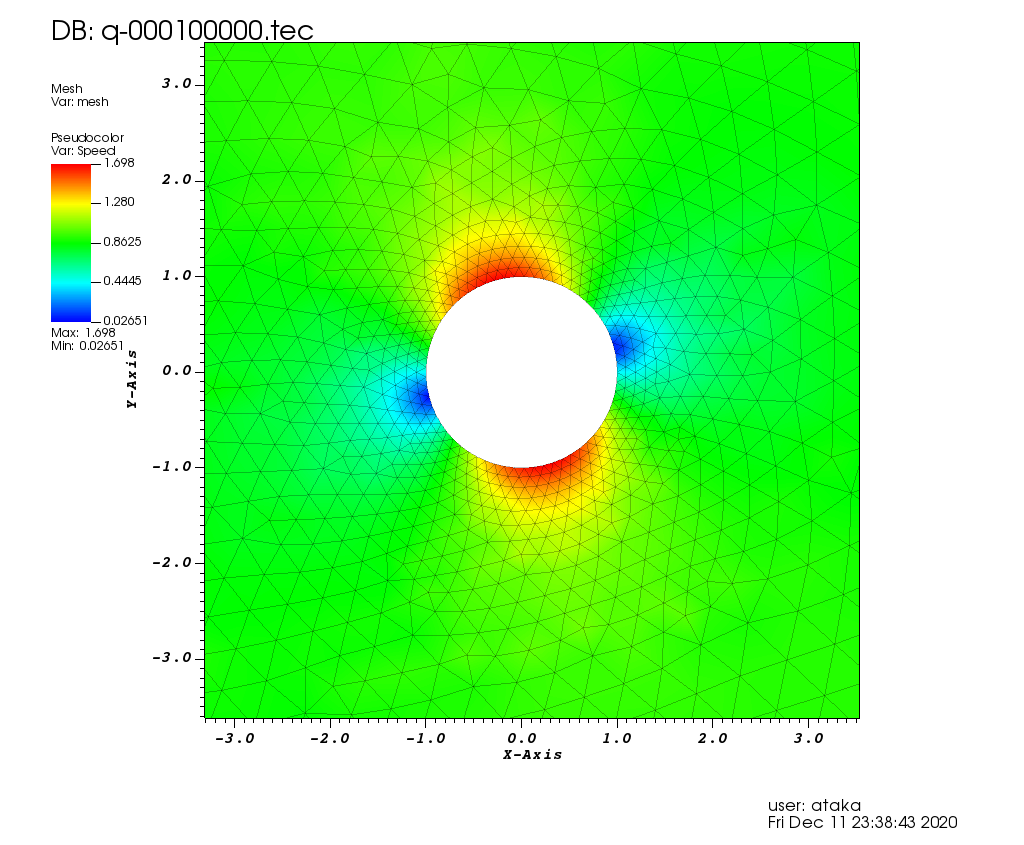
\includegraphics[height = 10cm]{graph/15deg/Cylinder_15angle_speed0001.png}
	\caption{Potential flow over a circular cylinder at $\alpha=15$ calculated by FV method.}
    \label{fig:q1p}
\end{figure}

According to the boundary conditions mentioned in Section \ref{section:intro}, FV fortran code
is completed. Afterwards, flowfield around a cylinder calculated using the unstructured grid provided.

\subsection{Flowfield Around A Cylinder with Different Angle of Attacks}
\begin{figure} [ht]
	\centering
	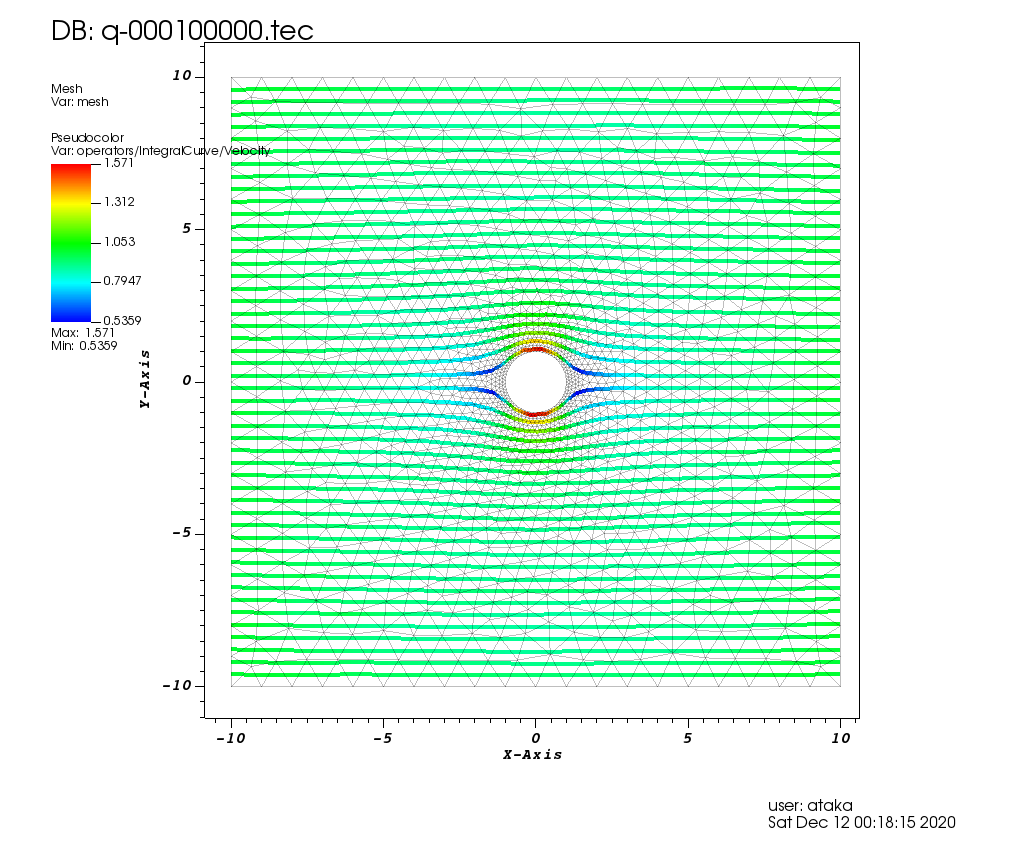
\includegraphics[height = 10cm]{graph/0deg/Cylinder_0angle_streamline0000.png}
	\caption{Streamlines over a circular cylinder at $\alpha=0$ calculated by FV method.}
    \label{fig:q2st0}
\end{figure}
\begin{figure} [ht]
	\centering
	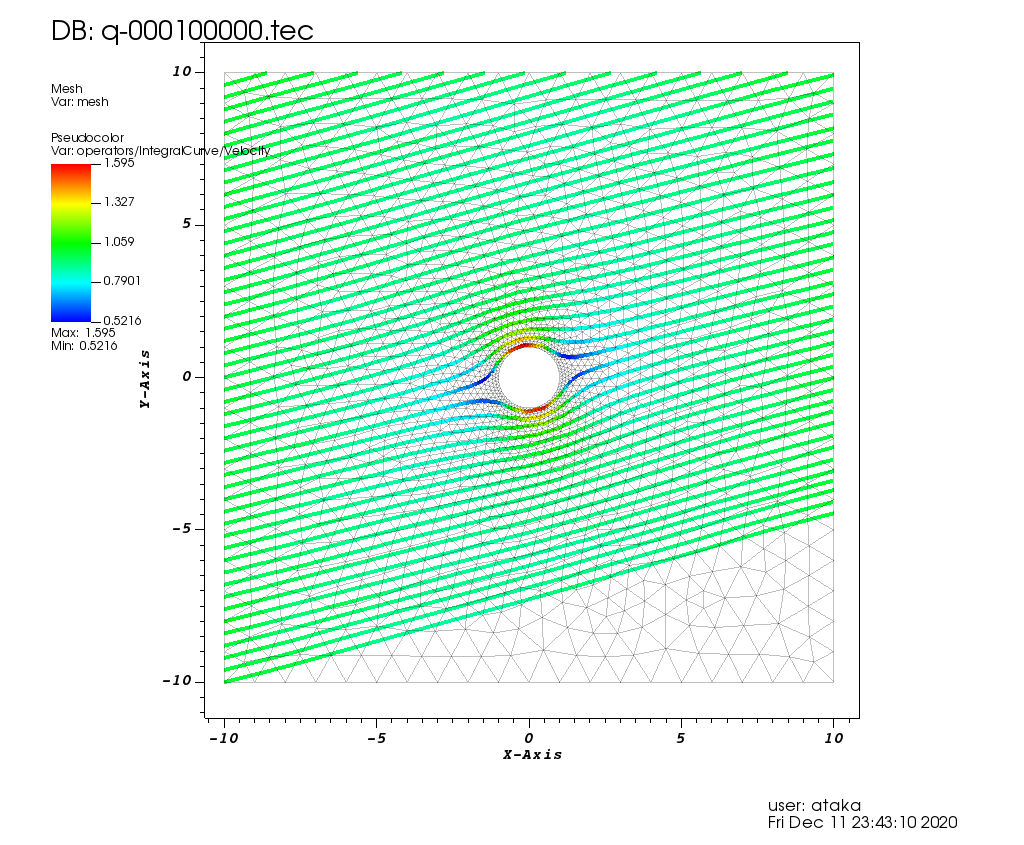
\includegraphics[height = 10cm]{graph/15deg/Cylinder_15angle_streamline0000.png}
	\caption{Streamlines over a circular cylinder at $\alpha=15$ calculated by FV method.}
    \label{fig:q2st15}
\end{figure}
\begin{figure} [ht]
	\centering
	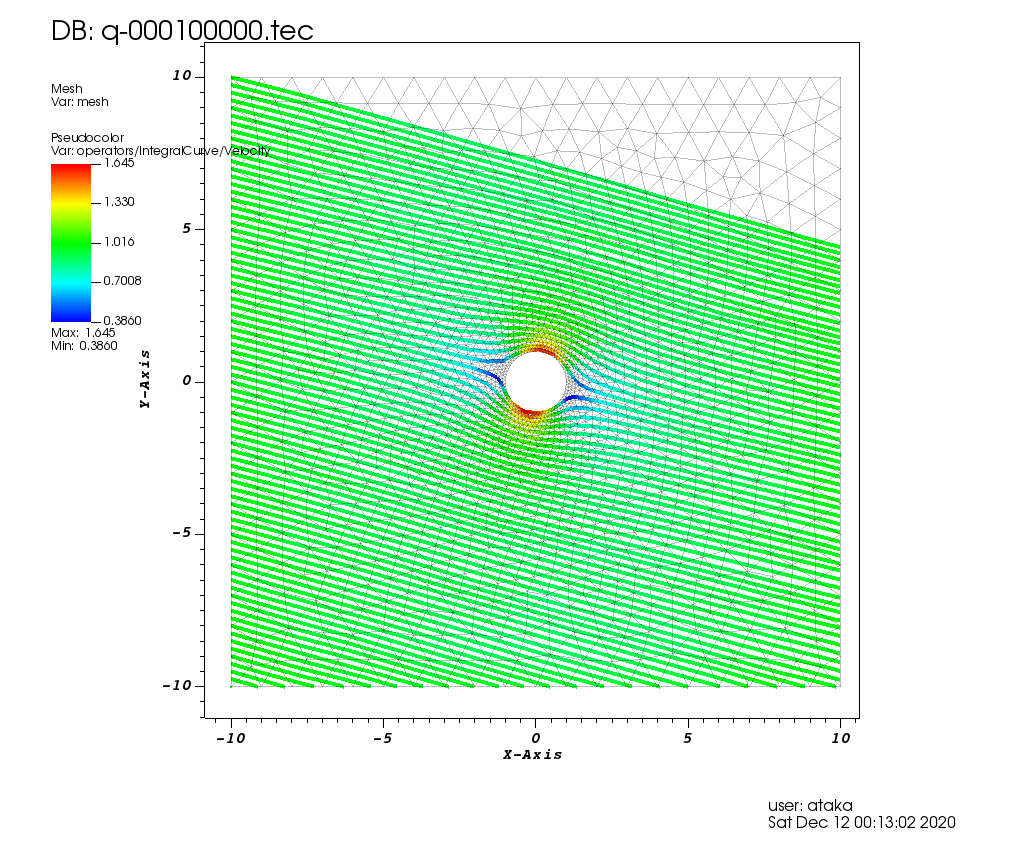
\includegraphics[height = 10cm]{graph/neg15deg/Cylinder_neg15angle_streamline0000.png}
	\caption{Streamlines over a circular cylinder at $\alpha=-15$ calculated by FV method.}
    \label{fig:q2st-15}
\end{figure}
In Figure \ref{fig:q2st0},\ref{fig:q2st15},and \ref{fig:q2st-15}, it can be observed that streamlines 
are parallel and horizontal lines far from cylinder. It can be named as Farfield boundary condition. 
However, as approached the cylinder, streamlines are squeeze. Streamlines do not across each other 
and over the cylinder. Also, no penetration is observed since normal component of velocity at the 
surface of cylinder is equal to zero. It can be called as wall boundary condition. 
\begin{figure} [ht]
	\centering
	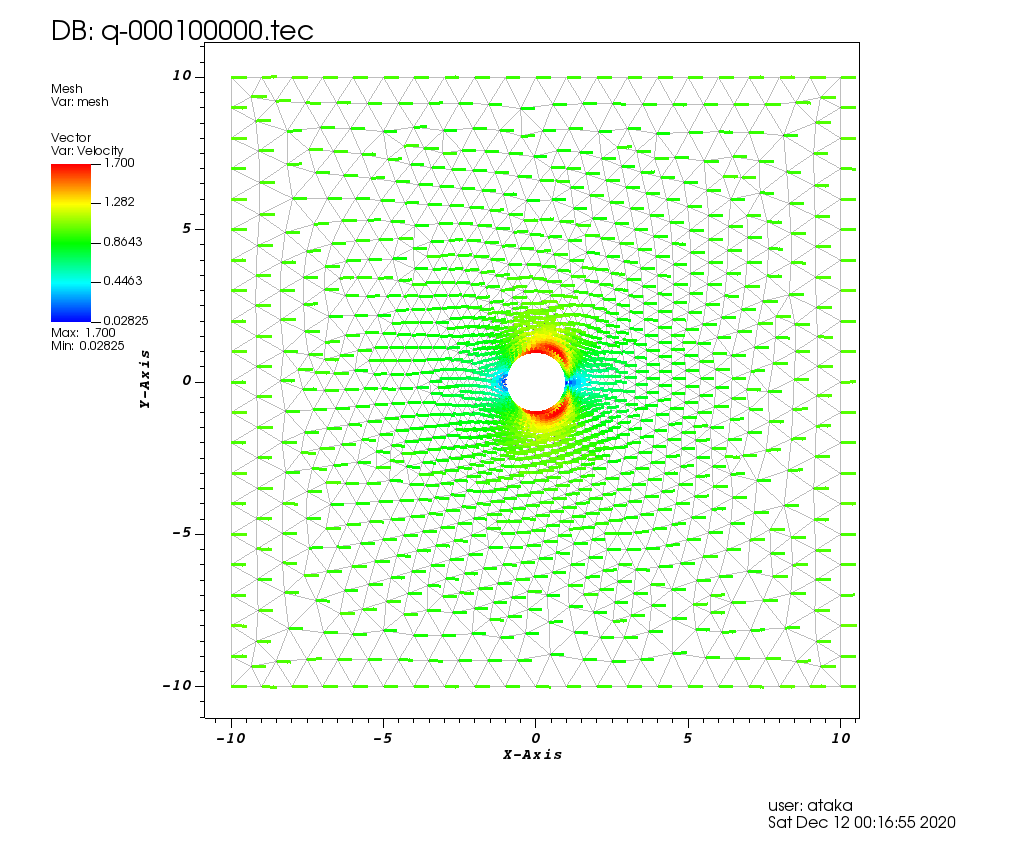
\includegraphics[height = 10cm]{graph/0deg/Cylinder_0angle_vector0000.png}
	\caption{The velocity vectors over a circular cylinder at $\alpha=0$ calculated by FV method.}
    \label{fig:q2v0}
\end{figure}
\begin{figure} [ht]
	\centering
	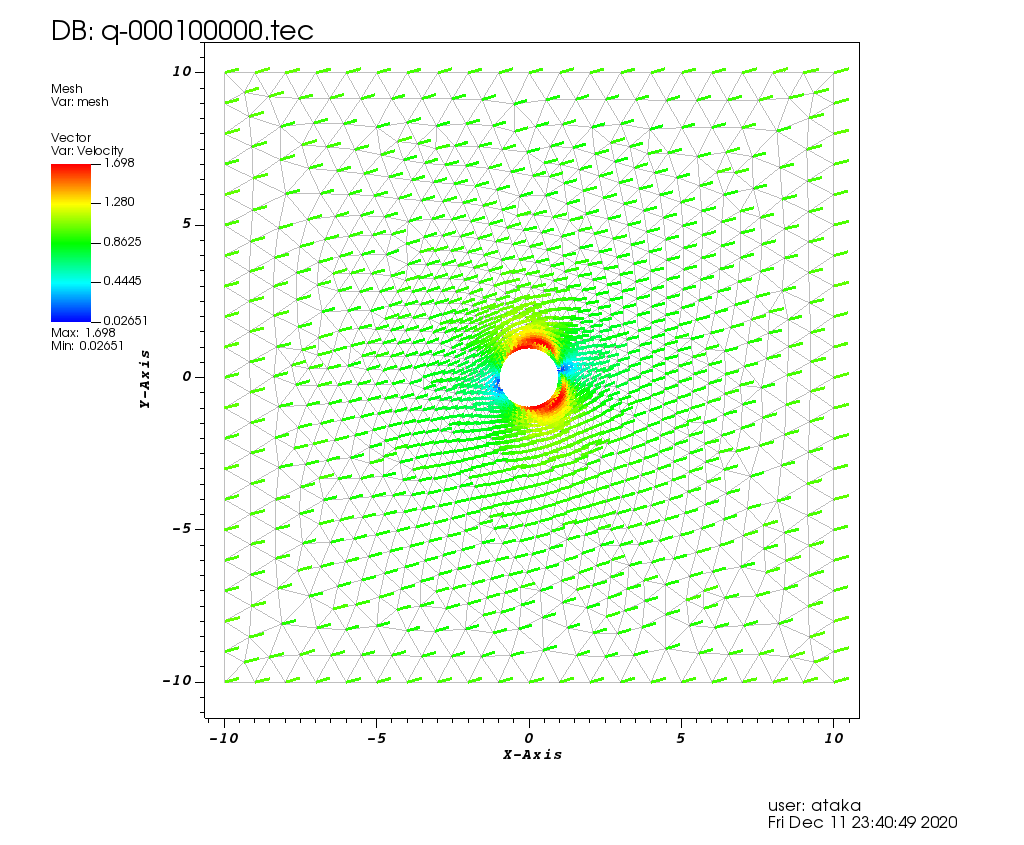
\includegraphics[height = 10cm]{graph/15deg/Cylinder_15angle_vector0000.png}
	\caption{The velocity vectors a circular cylinder at $\alpha=15$ calculated by FV method.}
    \label{fig:q2v15}
\end{figure}
\begin{figure} [ht]
	\centering
	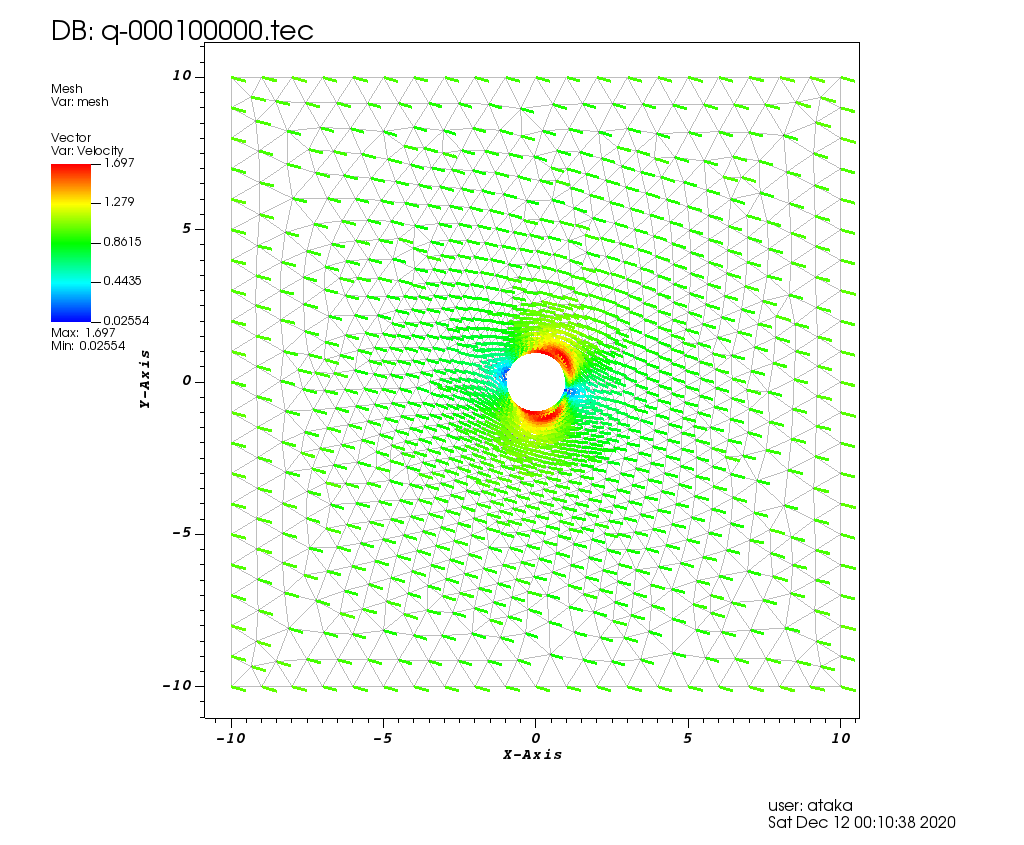
\includegraphics[height = 10cm]{graph/neg15deg/Cylinder_neg15angle_vector0000.png}
	\caption{The velocity vectors a circular cylinder at $\alpha=-15$ calculated by FV method.}
    \label{fig:q2v-15}
\end{figure}
According to Figure \ref{fig:q2v0},\ref{fig:q2v15},and \ref{fig:q2v-15}, velocity vectors have the 
same direction, and magnitudes far from cylinder. This is satisfies the Farfield boundry condition.
Also, the velocity vectors near the cylinder is tangent to the boundary. On the front and back of the 
cylinder, the direction of the velocity vector is too close to normal of surface. However, the 
magnitude of velocity is too small. Because normal components of velocity are zero at the boundary.





\section{Conclusion}

\end{document}